\chapter{Metaprogramming in Kotlin}\label{chapter:metaprogramming}
A typical program computation can be summarized as follows: it reads data as input, computes that data and generates an output.\newline
Metaprograms\footnote{\url{https://devopedia.org/metaprogramming}} are able to take as input another program, sometimes even the metaprogram itself, manipulate it and return a new version of it expressing a modified behavior.\newline 
In Figure~\ref{fig:programming_vs_metaprogramming} it is shown this difference with a representation of a simple program which transforms the input data, and a metaprogram which, on the other hand, modifies an entire input program generating an output program.
\begin{figure}[ht!]
    \centering
    \subfloat[\centering Simple program]{{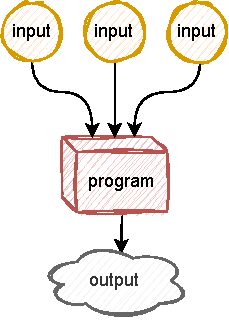
\includegraphics[scale=1.3]{document/chapters/2-metaprogramming/images/programming_vs_metaprogramming-programming.pdf} }}
    \qquad
    \subfloat[\centering Metaprogram]{{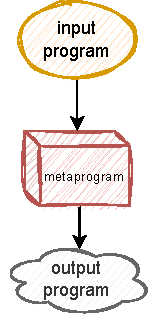
\includegraphics[scale=1.3]{document/chapters/2-metaprogramming/images/programming_vs_metaprogramming-metaprogramming.pdf} }}
    \caption{Representation of an execution of a simple program compared to a metaprogram}
    \label{fig:programming_vs_metaprogramming}
\end{figure}

Metaprogramming in Kotlin\footnote{\url{https://www.droidcon.com/2022/04/28/meta-programming-with-kotlin-for-android/}} is a powerful feature that allows for the manipulation and generation of code at compile time. The possible benefits of this technique are:
\begin{itemize}
    \item \textbf{Code generation}: it generates repetitive or boilerplate code automatically, reducing the amount of code that needs to be written and maintained by hand. Consequently, this can increase code readability and maintainability, as well as reducing the risk of introducing bugs or errors, that can be easily done by humans during the executions of repetitive tasks;
    \item \textbf{Readability}: it provides a higher level of abstraction, allowing to abstract away complex logic and make code more readable and easier to understand. This can also help to simplify the implementation of elaborated algorithms and data structures;
    \item \textbf{Reusability}: by generating code automatically, it is possible reuse the same logic across multiple parts of applications, increasing overall code reuse and maintainability;
    \item \textbf{Supports Domain-Specific Languages} (DSLs): it enables to create custom domain-specific languages (DSLs) that are optimized for specific tasks or use cases, which can help to simplify complex operations and make the code more readable and intuitive;
    \item \textbf{Custom annotations}: it allows creating custom annotations, which can be used to provide additional information about the code and to automate tasks such as code generation. This can improve code quality and make it easier to understand intentions and goals behind the code.
\end{itemize}

The main cost that has to be paid when dealing with metaprogramming is the increased \textbf{language complexity}.

\section{Metaprogramming techniques}
A multitude of different techniques can be used in Kotlin in order to create metaprograms. In the following sections the main approaches provided by Kotlin are going to be analyzed in details, in order to give an overview of the possible alternatives when coming into terms with metaprogramming.

\subsection{Annotations}\label{section:annotation}
Annotations\footnote{\url{https://kotlinlang.org/docs/annotations.html}} in Kotlin are a type of metadata that can be added to provide additional information about the code, as well as to automate certain tasks.

To create a custom annotation in Kotlin, first it is necessary to declare the annotation type, using the \textbf{annotation} keyword, as shown in the snippet of code in Listing~\ref{code:kotlin_annotations_creation}.
\begin{lstlisting}[caption={Example of creation of a custom annotation in Kotlin}, language=Kotlin, captionpos=b, label={code:kotlin_annotations_creation}]
annotation class MyAnnotation
\end{lstlisting}

Kotlin provides the option to use additional attributes by annotating the annotation class with \textbf{meta-annotation}. The available meta-annotation alternatives are:
\begin{itemize}
    \item \textbf{@Target}: it is used to specify the elements that can be annotated, which can be classes, functions, properties and expressions;
    \item \textbf{@Retention}: it defines if an annotation is stored in the compiled class files and if it is visible at runtime using reflections;
    \item \textbf{@Repeatable}: it allows an annotation to be used on the same element multiple times;
    \item \textbf{@MustBeDocumented}: it can be used when the annotation is part of a public API, and it must be included in the generated API documentation.
\end{itemize}

For example, this is a possible custom annotation that uses meta-annotation:
\begin{lstlisting}[caption={Example of custom annotation with meta-annotations in Kotlin}, language=Kotlin, captionpos=b, label={code:kotlin_annotations_customization}]
@Target(AnnotationTarget.CLASS, AnnotationTarget.FUNCTION)
@Retention(AnnotationRetention.RUNTIME)
annotation class MyAnnotation
\end{lstlisting}
In this snippet of code in Listing~\ref{code:kotlin_annotations_customization}, the \textbf{@Target} annotation specifies the elements that the annotation can be applied to, in this case either classes or functions. The \textbf{@Retention} annotation refers to the retention policy, which determines that the annotation is available at runtime.

Annotations can be used to provide metadata, such as the purpose of a function, the intended usage of a class, or the preferred behavior of a method. One possible use case is to use annotations to specify that a certain method should only be called on a background thread, or that a certain class is serializable.

Another feature provided by annotations, which is considered metaprogramming, is the possibility to use them to automate tasks, such as code generation. For example, annotations can be used to automatically generate code for serializing and deserializing objects.

It is possible to use the annotation in the code by placing the \textbf{@} (at) symbol, followed by the annotation type before the element that is going to be annotated, such as a class, function, or property.\newline
The snippet of code reported in Listing~\ref{code:kotlin_annotations_usage} shows how to actually use a custom annotation, specifically the one created in Listing~\ref{code:kotlin_annotations_customization}.
\begin{lstlisting}[caption={Example of usage of a custom annotation in Kotlin}, language=Kotlin, captionpos=b, label={code:kotlin_annotations_usage}]
@MyAnnotation
class MyClass

@MyAnnotation
fun myFunction() {
    val myVariable = 42
}
\end{lstlisting}
In this example, the \textbf{MyAnnotation} annotation is applied to both a class and a function. The annotations can be used by other code, either at compile time or at runtime, to provide additional information about the annotated elements.

\subsection{KSP}\label{section:ksp}
KSP stands for \textbf{Kotlin Symbol Processing}, and it is an API that can be used to build lightweight compiler plugins\footnote{\url{https://kotlinlang.org/docs/ksp-overview.html}\label{ksp_footnote}}. It offers an easy compiler plugin API that takes advantage of Kotlin's capabilities, but it keeps the learning curve low.

KSP has been developed as an alternative technology to \textbf{kapt}\footnote{\url{https://kotlinlang.org/docs/kapt.html}}, which was used to allow annotation processing. Currently, \textit{kapt} is in maintenance mode, meaning that it is being kept up-to-date with the new Kotlin and Java releases, but without adding any features.\newline
In comparison to \textit{kapt}, annotation processors that utilize KSP can be executed two times faster.

Kotlin Symbol Processing is a feature of the Kotlin compiler that allows to manipulate the code at compile time by processing the symbols contained in the code. As a consequence of that, it is possible to write metaprogramming code that analyzes, transforms, and generates other code, without the need to access the code at runtime.\newline
KSP reads the source code, generates new modules, and during the compilation the Kotlin compiler uses the original code and the generated source without distinctions, as it is shown in Figure~\ref{fig:ksp_diagram}, creating one executing program.

\begin{figure}[!ht]
    \centering
    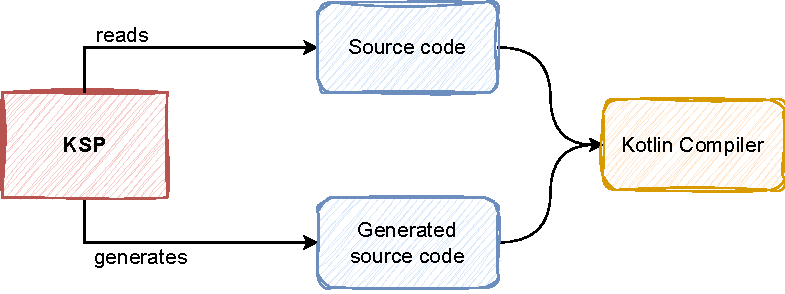
\includegraphics[scale=1]{document/chapters/2-metaprogramming/images/ksp_diagram.pdf}
    \caption{Representation of KSP behavior}
    \label{fig:ksp_diagram}
\end{figure}

This API allows processing Kotlin programs in a native way, with an understanding of Kotlin-specifc features, which includes extension functions, local functions and declaration-site variance. The API also models types explicitly, enabling type checking.

KSP models the structure of Kotlin programs, making class declarations, class members, functions and parameters accessible for processing, while elements such as if blocks and for loops are not.\newline
It can also be seen as a preprocessor framework, making a KSP plugin a symbol processor that follow three main steps:
\begin{enumerate}
    \item It analyzes the source program and its resources;
    \item It generates an output, which might be code or in another form;
    \item Finally, the Kotlin compiler compiles the source program with the generated output.
\end{enumerate}

Differently from a typical compiler plugin, KSP restricts processors from modifying the source code, as it is considered read-only. This choice can be justified by the intention to prevent confusion that may arise from a plugin that modifies the language semantics.

The source code, from the KSP perspective looks like this when being analyzed:
\begin{lstlisting}[caption={The source code from KSP perspective}, captionpos=b, label={code:ksp_source_code}]
KSFile
  packageName: KSName
  fileName: String
    declarations: List<KSDeclaration>
      KSClassDeclaration //class, interface, object
        simpleName: KSName
        qualifiedName: KSName
        containingFile: String
        typeParameters: KSTypeParameter
        parentDeclaration: KSDeclaration
        classKind: ClassKind
        primaryConstructor: KSFunctionDeclaration
        superTypes: List<KSTypeReference>
        //contains inner classes, functions, properties
        declarations: List<KSDeclaration>    
\end{lstlisting}
The Listing~\ref{code:ksp_source_code}\footref{ksp_footnote} shows the data structure that is accessible using KSP. Specifically, in this code it is contained a class declaration (\textit{KSClassDeclaration}), and it is possible to get its name, type, parameters, inner declarations, and so on.\newline
This representation allows to have a complete overview of the code structure.

KSP expects two elements to be implemented: the \textbf{SymbolProcessorProvider} and the \textbf{SymbolProcessor}.\newline
The \textit{create} function is invoked when KSP creates an instance of the \textit{SymbolProcessor}: this means that, without the \textit{SymbolProcessorProvider}, it would not be possible to instantiate a \textit{SymbolProcessor}. The \textit{SymbolProcessorProvider} is separated from the \textit{SymbolProcessor} to allow more freedom during the development.
The \textit{SymbolProcessorProvider} interface is defined like shown in Listing~\ref{code:symbol_processor_provider_interface}\footref{ksp_footnote}.
\begin{lstlisting}[caption={SymbolProcessorProvider interface}, language=Kotlin, captionpos=b, label={code:symbol_processor_provider_interface}]
interface SymbolProcessorProvider {
    fun create(environment: SymbolProcessorEnvironment):
        SymbolProcessor
}
\end{lstlisting}

In Listing~\ref{code:symbol_processor_interface}\footref{ksp_footnote} is shown the interface of the \textit{SymbolProcessor}.\newline
The only function that needs to be overridden is \textit{process}, which is typically used to read files and pass the elements to the visitors.
\begin{lstlisting}[caption={SymbolProcessor interface}, language=Kotlin, captionpos=b, label={code:symbol_processor_interface}]
interface SymbolProcessor {
    fun process(resolver: Resolver): List<KSAnnotated>
}
\end{lstlisting}
The \textit{Resolver} is the entry point of the functionalities provided by KSP: it can be used, for example, to get all the files of the source code, the symbols with annotation, a class, or a function declaration by name.\newline
As many other compiler related APIs, KSP supports the \textbf{visitor pattern}, allowing to examine each element in an object-oriented way.\newline
For example, the code in Listing~\ref{code:ksp_visitor}\footref{ksp_footnote} reports an implementation of a visitor that inspects the declarations and collects the function names in a list.
\begin{lstlisting}[caption={Visitor that collects function declarations}, language=Kotlin, captionpos=b, label={code:ksp_visitor}]
class FindFunctionsVisitor: KSTopDownVisitor<Unit, Unit>() {
    override fun visitFunctionDeclaration(
        function: KSFunctionDeclaration,
        data: Unit
    ) {
        functions.add(function.toString())
    }
}
\end{lstlisting}

In conclusion, one of the biggest strength of KSP is that it provides an API built on top of the compiler plugin: for this reason, it is able to hide the compiler changes, minimize maintenance efforts, and its API makes possible to implement a light-weight compiler plugin without the complexities and the knowledge required to create a real compiler plugin.\newline
On the other hand, since the goal of KSP is to be a simple solution for common problems, it comes with some limitations \footnote{\url{https://kotlinlang.org/docs/ksp-why-ksp.html}}:
\begin{itemize}
    \item it can not examine expression-level information;
    \item it can not modify the source code, but it can only generate new code;
    \item it is not integrated within the IDE, meaning that the IDE does not have any information about the code generated.
\end{itemize}

\subsection{Kotlin compiler plugins}\label{section:compiler_plugin_explanation}
Kotlin compiler plugins\footnote{\url{https://resources.jetbrains.com/storage/products/kotlinconf2018/slides/5\_Writing\%20Your\%20First\%20Kotlin\%20Compiler\%20Plugin.pdf} \label{compiler_plugin_slides_footnote}} are a way to extend the functionalities of the Kotlin compiler by adding custom processing to the compilation. This means that the compiler plugin code runs at compile-time, and, since this is a feature of \textit{kotlinc}, it only works on Kotlin source code.

Compiler plugins allow automating tasks and enforce coding standards. For example, they can be used to generate boilerplate code, such as accessor methods, or to enforce specific naming conventions or coding styles. Compiler plugins can also be used to perform code analysis and modification, such as adding custom checks and warnings, or refactoring the code automatically.

Kotlin compiler provides a powerful API, which makes it possible to even modify the internals of functions and classes. This enables to solve metaprogramming problems that were impossible using annotation processors, for example with KSP. Another advantage is that compiler plugins work on every Kotlin target, without having to write multiple plugins.

However, it is important to be aware of the potential downsides of using Kotlin compiler plugins. One of the main cons is that in order to write even a really simple plugin, it is necessary to have compiler background knowledge. Because of the high learning curve, it is important to consider very carefully if it is necessary to develop a plugin. The investment of time and work can be significant and, beside understanding how a compiler plugin works, it is necessary to develop:
\begin{itemize}
    \item \textbf{An IntelliJ plugin}: whenever they are used synthetics members, such as functions that are going to be created by the plugin at compile time, the IntelliJ plugin is used to avoid errors highlights, making the IDE understand what is going on;
    \item \textbf{A Gradle or Maven plugin}: in order to make the user able to use and configure the compiler plugin;
    \item \textbf{The actual compiler plugin}.
\end{itemize}

Moreover, compiler plugins can slow down the compilation process and make it more complex. Additionally, this can cause compatibility issues with different versions of the Kotlin compiler, and may require significant effort to maintain and update. It is also worth mentioning that because compiler plugins modify the behavior of the compiler, they can potentially introduce bugs and cause compatibility issues with other plugins.

Finally, another aspect that must be taken in consideration is the fact that the Kotlin compiler API is not documented. This means that working with it and understanding the functions' behaviors is not an easy task, and it requires even more time.

A Kotlin compiler plugin architecture is organized as shown in Figure~\ref{fig:kotlin_compiler_plugin_architecture}\footref{compiler_plugin_slides_footnote}.

\begin{figure}[!ht]
    \centering
    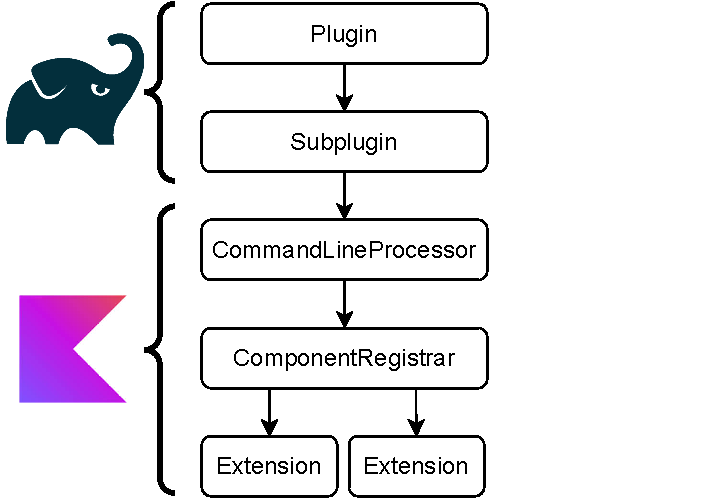
\includegraphics[scale=1]{document/chapters/2-metaprogramming/images/kotlin_compiler_plugin_architecture.pdf}
    \caption{The Kotlin compiler plugin architecture}
    \label{fig:kotlin_compiler_plugin_architecture}
\end{figure}

Two different modules can be distinguished in the architecture: a Gradle module and a Kotlin module.

The \textbf{Gradle module} is a wrapper for the Kotlin module, and it is an entry point for Gradle. The Gradle module is composed by:
\begin{itemize}
    \item \textbf{plugin}: this part is unrelated to Kotlin, and it is based on the Gradle API. It provides an entry point from a \textit{build.gradle} script, and it makes possible to configure the plugin via Gradle extensions;
    \item \textbf{subplugin}: this is the bridge that allows the interaction between Gradle and the Kotlin APIs. It reads the Gradle extension options and defines the compiler plugin's identifier, which is a unique key used in order to avoid collision with other plugins. The subplugin defines also the location of the compiler plugin artifact, which is going to be used to download it at compile time. The location can be local or a Maven coordinate.
\end{itemize}

\noindent The \textbf{Kotlin module} is dived in three main parts:
\begin{itemize}
    \item \textbf{CommandLineProcessor}: the options created in the Gradle subplugin are loaded and used by the CommandLineProcessor. Whenever a Kotlin program is launched, \textit{kotlinc} is invoked and the arguments that are set in the subplugin are passed to the Kotlin compiler;
    \item \textbf{ComponentRegistrar}: it registers the extension components, which are going to be used when the project is compiling;
    \item \textbf{Extensions}: they are used to actually generate code. There are a lot of different extensions, which are used based on the use case.
\end{itemize}

Since the components of a plugin architecture have been explained from a general point of view, it is now necessary to explain each element more in depth.\newline
Specifically, the following sections are organized as follows: Section~\ref{section:gradle_plugin} introduces how to create a Gradle plugin necessary to use a compiler plugin, Section~\ref{section:kotlin_ir} goes into details of the \textbf{IR} (\textbf{I}ntermediate \textbf{R}epresentation) that is the foundation that makes a compiler plugin possible, in Section~\ref{section:compiler_plugin_basics} it is explained how to inspect and navigate Kotlin IR, in Section~\ref{section:compiler_plugin_advaced} are covered advanced features, such as how to build new elements and how to transform the Kotlin IR, and Section~\ref{section:compiler_plugin_example} brings all together, showing the highlights of a working example of a simple Kotlin compiler plugin.

\subsubsection{Gradle Plugin}\label{section:gradle_plugin}
A Gradle plugin\footnote{\url{https://docs.gradle.org/current/userguide/custom_plugins.html}} is typically used to handle a set of tasks that extend the project's capabilities.\newline
In the context of Kotlin compiler plugins, the Gradle plugin is responsible for:
\begin{itemize}
    \item Giving the \textbf{artifact coordinates} of the compiler plugin: this is used to download the artifact from Maven Central or another location, which might be a local submodule;
    \item Defining the \textbf{identification string} of the compiler plugin: used to avoid conflicts with other compiler plugins options, since the identification string of the plugin is used to separate the command line options;
    \item Translating the Gradle configuration to \textbf{command line options}.
\end{itemize}

In order to create the artifact coordinates and the ID it is possible to use the \textit{buildconfig} plugin\footnote{\url{https://github.com/gmazzo/gradle-buildconfig-plugin}}.
\begin{lstlisting}[caption={Example of a \textit{buildconfig} that creates the compiler plugin artifact}, language=Kotlin, captionpos=b, label={code:build_config_example}]
buildConfig {
    val project = project(":compiler-plugin")
    packageName(project.group.toString())
        buildConfigField("String", "KOTLIN_PLUGIN_ID", "\"${project.group}.${project.name}\"")
    ...
}
\end{lstlisting}
The code in Listing~\ref{code:build_config_example} shows how to create references to a subproject called \textit{compiler-plugin} and how to create the identification string, which is the concatenation of the project group and name. Similarly, it is possible to reference the name, the version and the project group of the compiler plugin, creating a unique reference to its artifact.

After creating the configuration just presented, it is possible to create the actual Gradle plugin, such as in Listing~\ref{code:gradle_plugin_example}. Gradle exposes an interface that is specifically created for Kotlin compiler plugins, which is called \textbf{KotlinCompilerPluginSupportPlugin}.
\begin{lstlisting}[caption={Gradle plugin class example}, language=Kotlin, captionpos=b, label={code:gradle_plugin_example}]
class GradlePlugin : KotlinCompilerPluginSupportPlugin {
    ...
}
\end{lstlisting}
From this class they can be defined the compiler artifact, the identification string and any needed extension. For example, a Gradle Extension can be used to accept a command line parameter that enable and disable the plugin.

Basically, the creation of a Gradle plugin when dealing with Kotlin compiler plugins is always the same, and it is based on the notions just discussed in this section.

\subsubsection{Kotlin IR}\label{section:kotlin_ir}
The Kotlin compiler is organized in two parts: the \textit{frontend} is used to analyze the code, and the \textit{backend} is the one that generates the executables.\newline
Kotlin used to have three different backends: Kotlin/JVM, Kotlin/JS and Kotlin/Native. These backends were used to generate JVM byte code, JavaScript and LLVM IR, which is the representation for Kotlin Native.

When the Kotlin/Native backend was first developed, it was based on a new infrastructure, which used an internal representation for Kotlin code\footnote{\url{https://blog.jetbrains.com/kotlin/2021/02/the-jvm-backend-is-in-beta-let-s-make-it-stable-together/}}. After its stabilization, Kotlin developers started to migrate the other two backends to the same representation. This allows to share the backend logic, and to have most of the feature and optimization done only once for all the targets. Moreover, the common backend infrastructure grants the possibility to create \textbf{multiplatform} compiler plugins.

\begin{figure}[!ht]
    \centering
    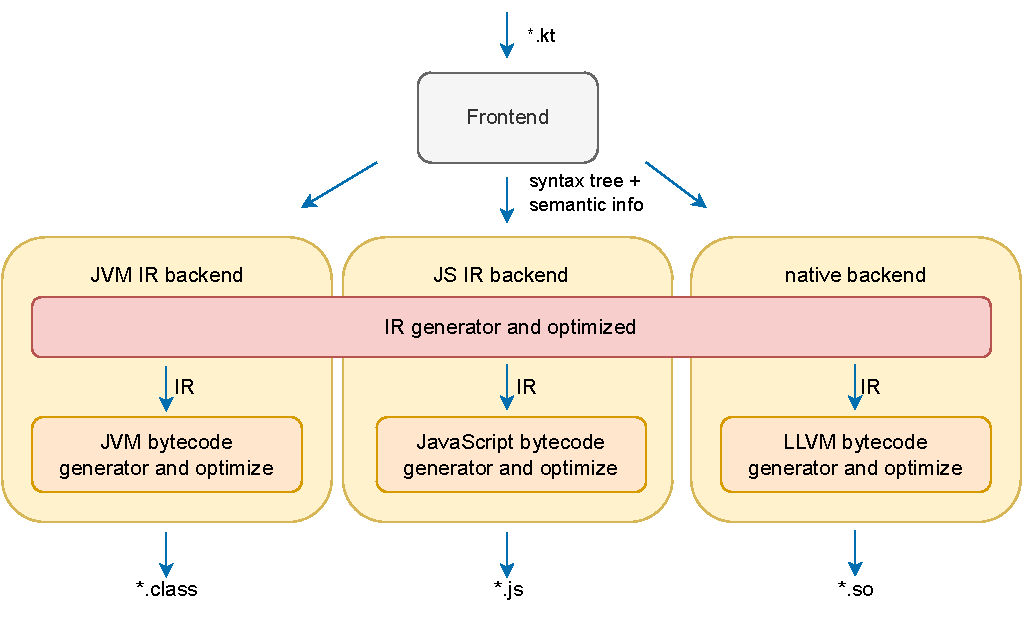
\includegraphics[scale=0.9]{document/chapters/2-metaprogramming/images/kotlin_compiler_plugin_ir_representation.pdf}
    \caption{The new Kotlin compiler backend that uses IR}
    \label{fig:kotlin_compiler_plugin_ir_representation}
\end{figure}

Currently, the structure of the compiler can be represented as in Figure~\ref{fig:kotlin_compiler_plugin_ir_representation}\footnote{\url{https://twitter.com/kotlin/status/1453741469148270593/photo/1}}: the frontend takes as input source file written in Kotlin, and then, each backend creates a syntax tree with all the information, using the IR representation. Only after this step, the code is transformed in the specific bytecode of each backend, which is different for each target.

The IR representation is an \textbf{abstract syntax tree} (\textbf{AST}). An AST\footnote{\url{https://dev.to/balapriya/abstract-syntax-tree-ast-explained-in-plain-english-1h38}} is a data structure that represents the abstract syntactic structure of a program. It is a tree representation of the source code, where each node in the tree corresponds to a construct in the source code. The nodes in the tree contain information about the construct, such as its type, location, and properties.\newline
For example, considering the simple snippet of pseudocode in Listing~\ref{code:ast_pseudocode}.
\begin{lstlisting}[caption={Pseudocode of a simple assignment and expression}, language=Kotlin, captionpos=b, label={code:ast_pseudocode}]
if (a < b) {
    x = a + b
} else {
    x = a - b
}
\end{lstlisting}
The AST that is generated from the code structure of Listing~\ref{code:ast_pseudocode} is shown in Figure~\ref{fig:ast_pseudocode_example}.
\begin{figure}[!ht]
    \centering
    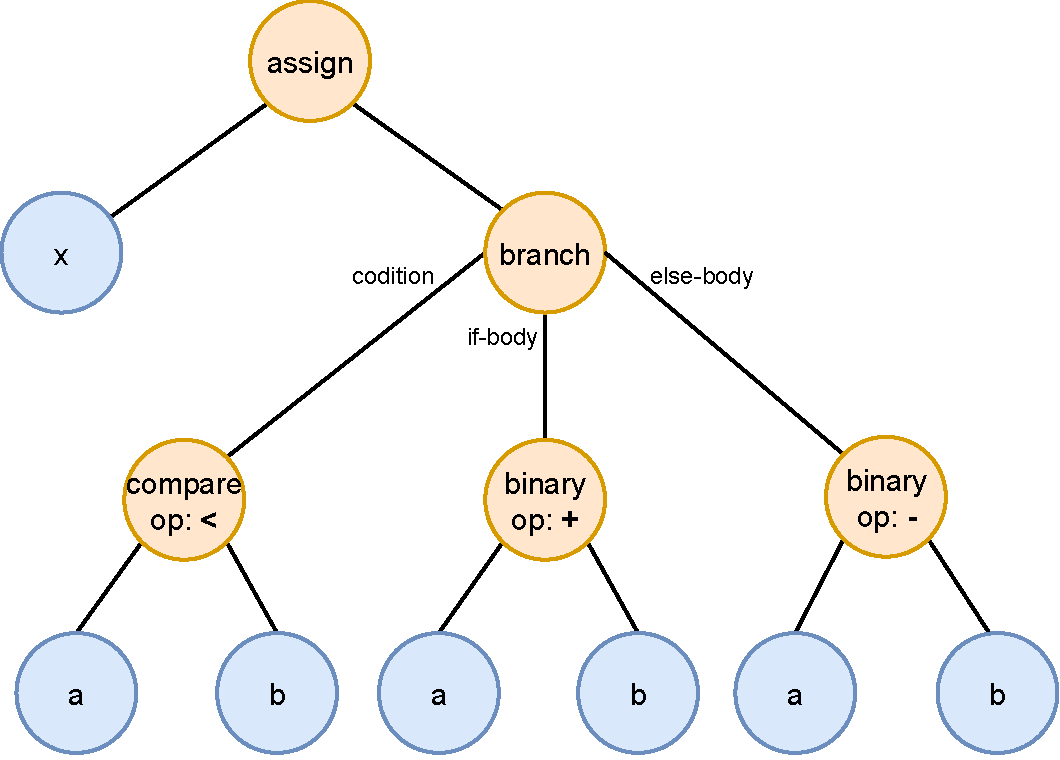
\includegraphics[scale=0.8]{document/chapters/2-metaprogramming/images/ast_pseudocode_example.pdf}
    \caption{The Abstract Syntax Tree of the source code in Listing~\ref{code:ast_pseudocode}}
    \label{fig:ast_pseudocode_example}
\end{figure}
Each node in the tree describes a construct in the source code. The root node represents the assignment of the result of the \textit{branch} expression to the variable \textit{x}. The \textit{branch} defines the conditional construct, and it has three children: the \textit{condition}, the \textit{if-body} and the \textit{else-body}. Each of these blocks is represented by a separate subtree, with \textit{<}, \textit{+} and \textit{-} nodes representing the comparison, addition and subtraction operations, respectively. The nodes \textit{a} and \textit{b} are the variables, that are used as operands of these operations.\newline
The condition node is crucial, because it is used to decide whether to evaluate the \textit{if-body} or the \textit{else-body}.

The AST is generated by a parser, which takes the source code as input and constructs the tree representation based on the syntax rules of the language. Once the AST is generated, it can be used for various purposes, such as type checking, code analysis, optimization, and code generation.\newline
An AST provides a more abstract and structured representation of the source code compared to the raw source code. This makes it easier to analyze and manipulate the code, as well as to automatically generate code or perform other tasks. For example, compilers use the AST to perform optimizations, such as constant folding, dead code elimination, and inlining, before generating machine code.

Hence, \textbf{Kotlin IR} (Intermediate Representation) backend is the part of the Kotlin compiler that generates a representation of the Kotlin code. This is used as the input for the next stage of the compilation, which can be either the code generator or another intermediate representation.

The IR backend is designed to provide a high-level, platform-agnostic representation of the Kotlin code, making it easier to target different platforms and architecture. The IR code is optimized for use by the code generator, reducing the number of intermediate representations required, and allowing for better optimization.

Kotlin IR backend is an important part of the Kotlin compiler as it enables the compiler to target different platforms, such as the JVM, JavaScript, and Native code, while still providing a high-level representation of the code. This makes it easier to maintain and evolve the compiler and provides a more flexible way to target new platforms in the future.

\subsubsection{Basics}\label{section:compiler_plugin_basics}
In order to be able to build a Kotlin compiler plugin it is necessary to understand how the Kotlin IR syntax tree looks like.

First, one important information is that every node in the tree implements the \textbf{IrElement} interface. IrElement has an extension function, called \textbf{dump()}, that allows to get as output the IR tree from any point.\newline
This feature is extremely useful when trying to generate code, because, in the case of errors, the exception thrown does not indicate what caused the problem. The message associated to a thrown exception just says the following:
\begin{lstlisting}[caption={Kotlin IR lowering Exception}, language=Kotlin, captionpos=b, label={code:ir_lowering_exception}]
org.jetbrains.kotlin.backend.common.BackendException: Backend Internal error: Exception during IR lowering
\end{lstlisting}
Typically, this is symptom of the generation of not well-formed elements, that are caught during compilation. This can be verified by writing the code that wants to be generated and comparing its \textit{dump()} output against the one created by the compiler plugin, finding the necessary changes that needs to be done.

For example, it is going to be analyzed the generated IR tree of this snippet of code:
\begin{lstlisting}[caption={Kotlin basic code to demostrate the Kotlin IR representation}, language=Kotlin, captionpos=b, label={code:kotlin_for_ir_tree}]
fun main() {
    println("test")
}
\end{lstlisting}

This is the complete Kotlin IR syntax tree that is generated from the source code of Listing~\ref{code:kotlin_for_ir_tree}:
\begin{lstlisting}[caption={Kotlin IR tree of Listing~\ref{code:kotlin_for_ir_tree}}, captionpos=b, basicstyle=\small, label={code:kotlin_ir_tree_example}]
FILE fqName:<root> fileName:Main.kt
FUN name:main visibility:public modality:FINAL <> () returnType:kotlin.Unit
 BLOCK_BODY
  CALL `public final fun println (message: kotlin.String): kotlin.Unit [external] declared in kotlin.io' type=kotlin.Unit origin=null
   message: CONST String type=kotlin.String value="test"
\end{lstlisting}
The indentation of the IR allows to understand the relationship between each node, increasing its readability. In order to provide more clarity, they are going to be analyzed the most significant nodes of the IR.\newline
Starting from the following node:
\begin{lstlisting}[caption={Kotlin IR tree of the main function in Listing~\ref{code:kotlin_for_ir_tree}}, captionpos=b, label={code:kotlin_ir_tree_main_example}]
FUN name:main visibility:public modality:FINAL <> () returnType:kotlin.Unit
\end{lstlisting}
This represents the definition of the \textit{main()} function and the IR tree representation provides a lot of information about it:
\begin{itemize}
    \item \textbf{FUN} indicates that the current node is a declaration of a function;
    \item \textbf{name} is used to express how the function is called;
    \item \textbf{visibility} shows that the main function visibility is public;
    \item \textbf{modality} declares that main is final;
    \item \textbf{<>} refers to the fact that the function does not have a generic type;
    \item \textbf{()} means that main does not take parameters;
    \item \textbf{returnType} indicates that the return type of the main function is \textit{kotlin.Unit}.
\end{itemize}

The child of the function IR element is the initialization of its body, which is declared like this:
\begin{lstlisting}[caption={Kotlin IR tree of the body block of the main function in Listing~\ref{code:kotlin_for_ir_tree}}, captionpos=b, label={code:kotlin_ir_tree_main_body_init_example}]
BLOCK_BODY
\end{lstlisting}
When analyzing the IR tree, two different keywords are going to be found for bodies. The first one is \textbf{BLOCK\_BODY}, which is used in this specific case in Listing~\ref{code:kotlin_ir_tree_main_body_init_example}: this means that the body is expected to have multiple statements. The second one is \textbf{EXPRESSION\_BODY}, which is indicated when the body holds a single expression, such as a variable assignment.

Finally, the Listing~\ref{code:kotlin_ir_tree_main_body_example} shows the \textit{println()} function call and its parameter:
\begin{lstlisting}[caption={Kotlin IR tree of the body block content of the main function in Listing~\ref{code:kotlin_for_ir_tree}}, captionpos=b, label={code:kotlin_ir_tree_main_body_example}]
CALL `public final fun println (message: kotlin.String): kotlin.Unit [external] declared in kotlin.io' type=kotlin.Unit origin=null
  message: CONST String type=kotlin.String value="test"
\end{lstlisting}
Similarly to the \textit{FUN} keyword, \textbf{CALL} is used to indicate that a function is being called. Specifically, it declares the call of the \textit{println} function, alongside with information about where to find its declaration, which is in this case in \textit{kotlin.io}, since the print is a Kotlin library function. Moreover, the function has one parameter, which is called message. The second line in Listing~\ref{code:kotlin_ir_tree_main_body_example} gives all the details about it: it is a constant, defined by the \textbf{CONST} keyword, it is a \textit{String} and its value is \textit{test}.

Another basic feature that needs to be explained is how to actually visit the IR syntax tree from the code point of view. One key concept that is necessary to cover before diving into it is the \textbf{visitor design pattern}\footnote{\url{https://www.baeldung.com/java-visitor-pattern}\label{visitor_pattern_footnote}}.
\begin{figure}[!ht]
    \centering
    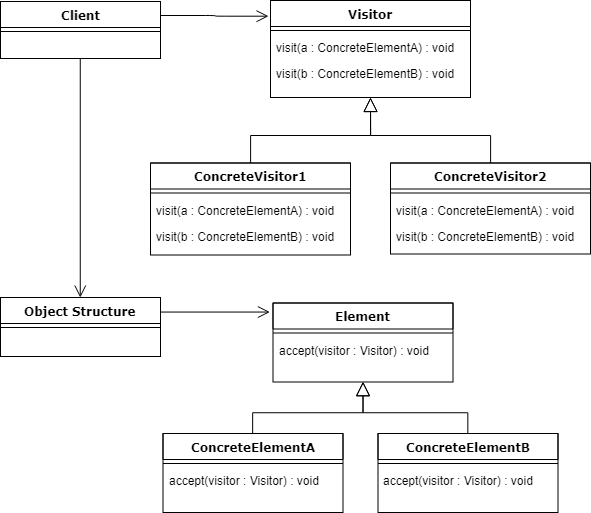
\includegraphics[scale=0.6]{document/chapters/2-metaprogramming/images/visitor_pattern_uml.png}
    \caption{The Visitor design pattern UML}
    \label{fig:visitor_uml}
\end{figure}
This is a behavioral design pattern which purpose is to add new operations to existing classes without modifying the classes themselves.\newline
The operation defined can be performed on elements of an object structure, which is defined in a separate class, called the \textbf{Visitor}, that implements the desired behavior. The elements of the object structure are updated to accept the Visitor instance, allowing it to traverse the structure and perform the operation on each element. The structure of the design pattern just described is reported in the UML in Figure~\ref{fig:visitor_uml}\footref{visitor_pattern_footnote}.

In the context of the Kotlin compiler, the visitor pattern is applied as in Figure~\ref{fig:visitor_uml_kotlin_compiler}. The \textit{IrElement} interface represents the object structure that needs to be visited. As anticipated previously in this section, this interface is implemented by all the node of the IR syntax tree, which means that every element can be visited through this pattern.\newline
\begin{figure}[!ht]
    \centering
    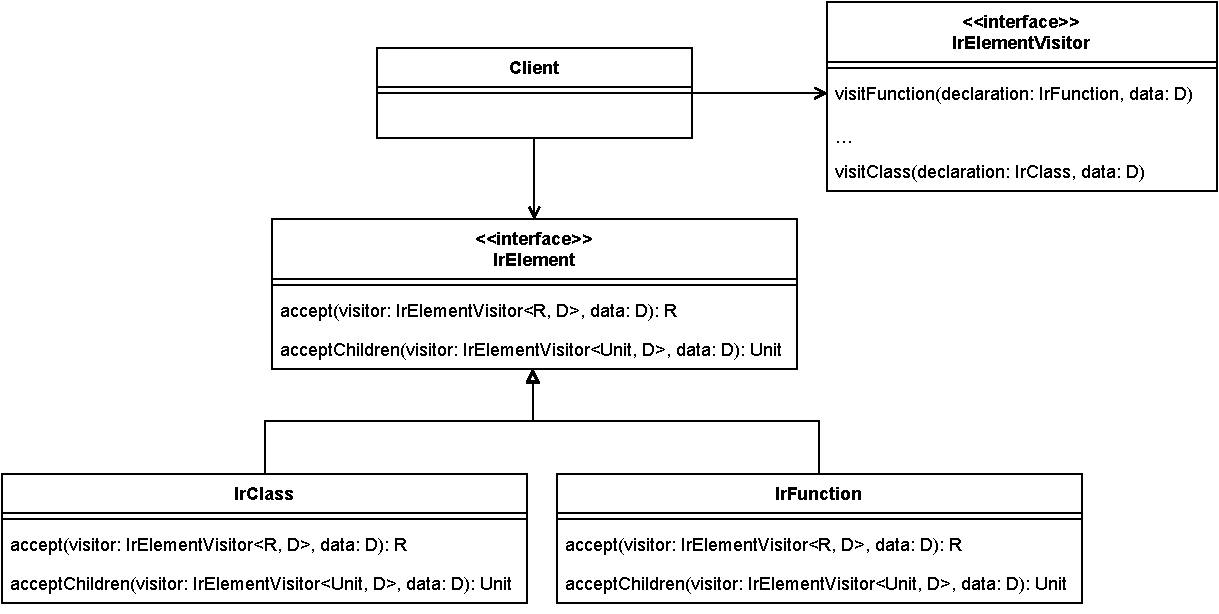
\includegraphics[scale=0.77]{document/chapters/2-metaprogramming/images/visitor_uml_kotlin_compiler.pdf}
    \caption{The Visitor design pattern UML applied in the Kotlin compiler plugin context in order to visit the IR syntax tree}
    \label{fig:visitor_uml_kotlin_compiler}
\end{figure}
For example, the two implementations of \textit{IrElement}, shown in Figure~\ref{fig:visitor_uml_kotlin_compiler}, are \textit{IrClass} and \textit{IrFunction}, which represents class declarations and function declarations respectively. A lot of other different elements that are not specified in the UML exists; this omission is done in order to increase its readability. Examples of the omitted elements are: \textit{IrConst} for constant, \textit{IrCall} for function calls, \textit{IrBranch} that includes if-else blocks, etc.\newline
The \textit{IrElement} has two functions that enable the visitor pattern that have two completely different behaviors:
\begin{itemize}
    \item \textbf{accept}: it allows the visit of only the current element. For example, if trying to visit a class, only the class element is going to be analyzed and returned;
    \item \textbf{acceptChildren}: this function implementation consists on calling the \textit{accept} function on each child of the current element, including itself.
\end{itemize}
Both functions possess two parameters, where the first one is the \textit{IrElementVisitor}, the second one is \textit{data}, which is used to pass information about the context to the IR visitor.\newline
The return type in the \textit{accept} function can be used to get as output the elements visited, and it is useful, for example, when the navigation aims to find a specific element. Otherwise, the return can just be set as \textit{Unit}.
\begin{lstlisting}[caption={Example of a custom visitor and a function that supports the collection of elements}, captionpos=b, language=Kotlin, label={code:accept_children_collect_example}]
class CustomVisitor(
  private val elements: MutableList<IrElement>
) : IrElementVisitor<Unit, Nothing?> {
  override fun visitElement(element: IrElement,data: Nothing?){
    elements.add(element)
    element.acceptChildren(this, data)
  }
}

fun collect(element: IrElement) = buildList<IrElement> {
  element.accept(CustomVisitor(this), null)
}
\end{lstlisting}
In the case of \textit{acceptChildren}, its return type is \textit{Unit}, which means that when visiting recursively the children of an element, no data can be returned. Whenever it is necessary to collect information from a recursive visitor, it is usually created a builder object that can be updated and then returned. In Listing~\ref{code:accept_children_collect_example}\footnote{\url{https://blog.bnorm.dev/writing-your-second-compiler-plugin-part-3}} the role of the \textit{collect} function is to create a mutable list that is updated on the visit of each child of the root element.

As previously said, the \textbf{IrElementVisitor} is the interface that has to be implemented in order to create a custom visitor. It requires two type parameters: the first one indicates the return type of the visit functions, the second one the type of the data that can be used to pass contextual information. The interface provides a lot of different visit methods, that can be used based on the wanted behavior. In Figure~\ref{fig:visitor_uml_kotlin_compiler} are reported \textit{visitFunction} and \textit{visitClass}, but other examples are \textit{visitBody}, \textit{visitVariable}, \textit{visitDeclaration}, etc.

The \textbf{IrElement} and the \textbf{IrElementVisitor}, with the understanding of the IR syntax tree, allows creating basic Kotlin compiler plugins, without modifying the existing source code.

\subsubsection{Advanced features}\label{section:compiler_plugin_advaced}
There are two advanced aspects that need to be introduced, which are the building of new IR elements and the transformation of the IR syntax tree.

In order to understand how to build IR elements, it is important to keep in mind that the Kotlin compiler entry point provides the \textbf{IrPluginContext}, which contains the information about the context of the plugin. This is a critical element because it can be used to obtain an instance of the \textbf{IrFactory}, which is a factory that can create IR elements, such as \textit{IrClass} for creating new classes or \textit{IrSimpleFunction} used for creating functions.\newline
\begin{lstlisting}[caption={Main function IR building by using the IrFactory}, captionpos=b, language=Kotlin, label={code:build_main_function_with_factory}]
pluginContext.irFactory.buildFun {
    name = Name.identifier("main")
    visibility = DescriptorVisibilities.PUBLIC
    modality = Modality.FINAL
    returnType = typeUnit
}        
\end{lstlisting}
For example, the code in Listing~\ref{code:build_main_function_with_factory}\footnote{\url{https://blog.bnorm.dev/writing-your-second-compiler-plugin-part-4}} shows how to use the factory to create a function called \textit{main} and that does not have a return type.

The factory can only be used to create new element declarations, so it is necessary another way in order to build statements and expressions. This is provided by the \textbf{IrBuilder} and by the \textbf{IrBuilderWithScope}, which is really convenient when, for example, a new statement is created in a specific function scope.

The transformation of the IR can be done similarly to the navigation seen in Section~\ref{section:compiler_plugin_basics}, but it is performed by another interface that extends \textit{IrElementVisitor}, which is called \textbf{IrElementTransformer}. The UML that shows the organization of the interfaces in this context can be seen in Figure~\ref{fig:transformer_uml_kotlin_compiler}.\newline
\begin{figure}[!ht]
    \centering
    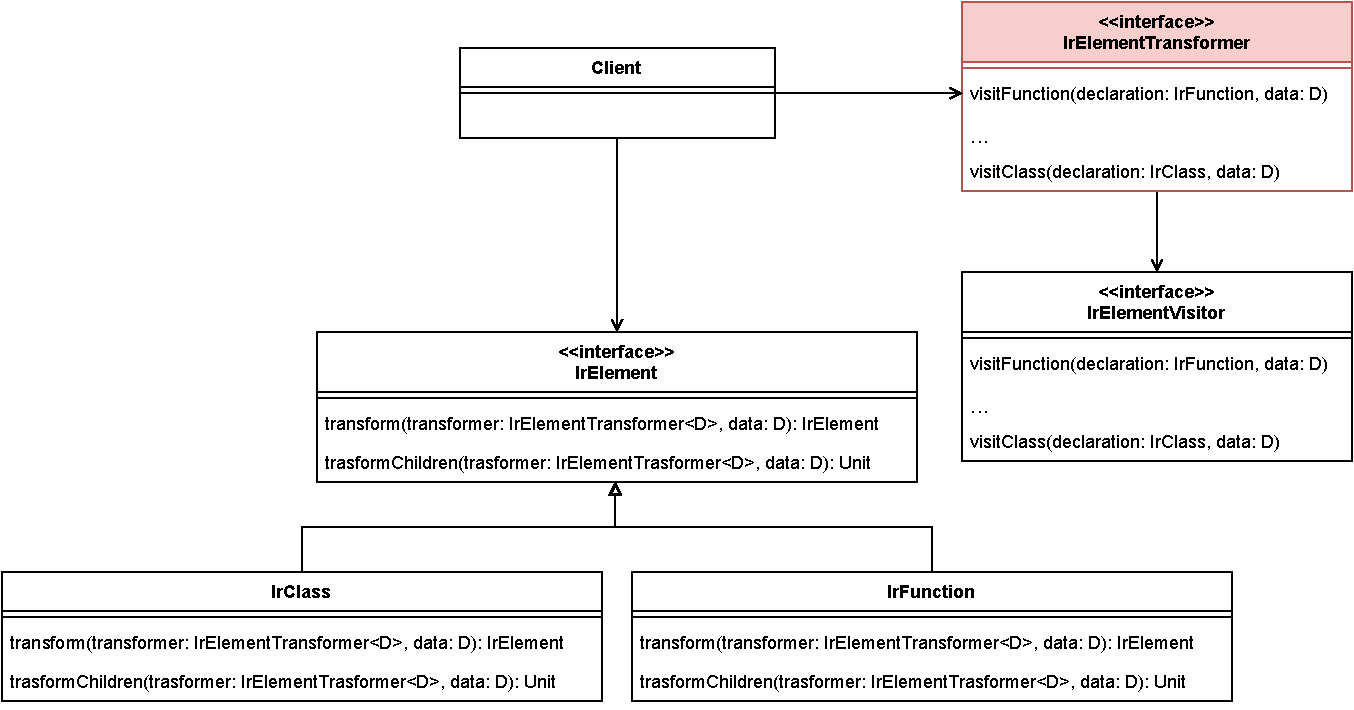
\includegraphics[scale=0.69]{document/chapters/2-metaprogramming/images/transformer_uml_kotlin_compiler.pdf}
    \caption{The Visitor design pattern UML applied in the Kotlin compiler plugin context in order to transform the IR syntax tree}
    \label{fig:transformer_uml_kotlin_compiler}
\end{figure}
Considering the \textit{IrElement}, there are two transforming functions, that matches the navigation functions:
\begin{itemize}
    \item \textbf{transform}: it is like the \textit{accept} function considered for the visiting of the IR tree, and it is used to transform only a specific element;
    \item \textbf{transformChildren}: similarly to \textit{acceptChildren}, it transforms recursively all the children of the element, including itself.
\end{itemize}
The \textit{IrElementTransformer} provides the same methods of the \textit{IrElementVisitor}, such as \textit{visitClass} and \textit{visitDeclaration}, but the return type is always set as the element itself. Basically, when wanting to transform a function it is sufficient to create an \textit{IrElementTransformer} and to override the \textit{visitFunction} method, implementing whatever transformation needed. For example the element can be modified  or created by using the \textit{IrFactory} or the \textit{IrBuilder}, or existing elements can be deleted.

As a whole, all these functionalities discussed constitute powerful tools that allow all kind of compile-time modifications, that can be encapsulated in a Kotlin compiler plugin.

\subsubsection{Example}\label{section:compiler_plugin_example}
The complexities involved in Kotlin compiler plugins, discussed in the previous sections, need a further exploration. For this reason, it has been developed a simple plugin\footnote{\url{https://github.com/ElisaTronetti/compiler-plugin-kmp}}, which aims to dive deeply into the details of basic and advanced features implementation.

For example, considering the following code:
\begin{lstlisting}[caption={Kotlin code without the modification of the compiler plugin created as an example}, captionpos=b, language=Kotlin, label={code:main_compiler_plugin_example}]
fun test() {
    println("Hello!")
}
    
fun main() {
    test()
}
\end{lstlisting}
When executing the code in Listing~\ref{code:main_compiler_plugin_example}, this is the result shown in the console:
\begin{lstlisting}[caption={Output of the execution of Listing~\ref{code:main_compiler_plugin_example} with the application of the compiler plugin created as an example}, captionpos=b, language=Kotlin, label={code:output_main_compiler_plugin_example}]
main declaration
test declaration
Hello!
\end{lstlisting}
The goal of this compiler plugin is to modify at compile time every function declaration, inserting a print of the function name. This means that after the compilation, the code in Listing~\ref{code:main_compiler_plugin_example} is going to be transformed as in the code in Listing~\ref{code:main_compiler_plugin_example_after_compilation}. The arrows added are used to identify the lines of code created by the compiler plugin.
\begin{lstlisting}[caption={Kotlin code with the modification of the compiler plugin created as an example}, captionpos=b, language=Kotlin, escapechar=\$, label={code:main_compiler_plugin_example_after_compilation}]
fun test() {
    -> println("test declaration")
    println("Hello!")
}

fun main() {
    -> println("main declaration")
    test()
}
\end{lstlisting}
One thing to notice is that, typically, the functions' names are not passed from compilation time to run time, this information would be usually lost. By the intervention of the plugin, that information is not lost, but it is inserted in the print function and shown to the user.

Moreover, the module of the project that contains the code that is going to use the compiler plugin is a \textbf{Kotlin Multiplatform} project. The reasons behind this choice are going to be explained afterwards in Section~\ref{section:technology_choices}, but this example is also a \textbf{proof of concept} of the feasibility of creating Kotlin compiler plugins for multiplatform projects.

This project example is composed by three submodules:
\begin{itemize}
    \item \textit{gradle-ir-plugin}: it creates the subplugin, identifying the location of the compiler plugin, which is in the same Gradle project but in a different submodule;
    \item \textit{compiler-ir-plugin}: the actual compiler plugin, that is going to be discussed in details;
    \item \textit{kmp-sample}: it is the Kotlin multiplatform project, which uses the Gradle plugin to include the compiler plugin;
\end{itemize}

Since the Gradle module is just based on mandatory  but standard settings, it is only going to be analyzed the compiler module.\newline
The first component of the compiler plugin is the \textbf{CommandLineProcessor}, which sets one command line option: when including the plugin to a project, it can be specified a boolean parameter that enables or disable the plugin, making it easier to use.\newline
The creation of this parameter consists on building an option using the \textit{CliOption} class, which is used to inform the compiler plugin what parameters to expect and what is their role. The option created for this example is shown in the code in Listing~\ref{code:cli_option_example}.
\begin{lstlisting}[caption={Creation of compiler option that enables or disables the plugin}, captionpos=b, language=Kotlin, label={code:cli_option_example}]
CliOption(
    optionName = ARG_ENABLED,
    valueDescription = "bool <true | false>",
    description = "If the compiler plugin should be applied",
    required = false
)
\end{lstlisting}

The entry point of the compiler plugin is the \textbf{ComponentRegistrar}. It checks whether the plugin is enabled or not, and, in case it is, it registers a generation extension, which is going to actually perform code changes. In the \textit{ComponentRegistrar} implementation, the function that perform this feature is the following:
\begin{lstlisting}[caption={Example of registration of extension if the plugin is enabled performed by the \textit{ComponentRegistrar}}, captionpos=b, language=Kotlin, label={code:component_registrar_example}]
override fun registerProjectComponents(
    project: MockProject,
    configuration: CompilerConfiguration
) {
    if (configuration.get(ARG_ENABLED)) {
        IrGenerationExtension.registerExtension(
            project,
            IrGenerationExtensionImpl()
        )
    }
}
\end{lstlisting}
In Listing~\ref{code:component_registrar_example} it is shown how to register the extension that is going to generate code. The \textbf{IrGenerationExtension} implemented method is \textit{generate}, and it is shown in Listing~\ref{code:generation_extension_example}.
\begin{lstlisting}[caption={Example of \textit{IrGenerationExtension} implementation of methos generate}, captionpos=b, language=Kotlin, label={code:generation_extension_example}]
override fun generate(
    moduleFragment: IrModuleFragment,
    pluginContext: IrPluginContext
) {
    val funPrintln = pluginContext.referenceFunctions(
        FqName("kotlin.io.println")
    ).first()

    moduleFragment.transform(
        TransformerImpl(pluginContext, funPrintln),
        null
    )
}
\end{lstlisting}
The \textit{generate} method just shown has two different purposes:
\begin{itemize}
    \item It aims to find the reference of the Kotlin print function, which is going to be used in the code generation. This is done by specifying the name of the function and its package, then it is going to be searched in the whole plugin context;
    \item It creates an instance of the transformer implementation, giving it as argument the plugin context and the print function found, which are all the information that is going to be used to modify the code.
\end{itemize}

The most important element of all, that actually perform the code transformation, is the \textbf{TransformerImpl}, which implements the \textbf{IrElementTransformer} interface.\newline
Since the modifications that needs to be achieved are applied to all the function declaration bodies, the \textit{visitFunction} needs to be overridden as reported in the code in Listing \ref{code:visit_function_declaration_example}, which works in the following way:
\begin{itemize}
    \item for each function declaration found in the context, verify if it has a body. For example, abstract declarations do not have a body;
    \item if a body is found, it modifies the declaration it passing it to the \textit{irDebug} function.
\end{itemize}

\begin{lstlisting}[caption={Example of \textit{visitFunction} implementation of the transformer, used to visit all the function declarations}, captionpos=b, language=Kotlin, label={code:visit_function_declaration_example}]
override fun visitFunction(
    declaration: IrFunction
): IrStatement {
    val body = declaration.body
    if (body != null) {
        declaration.body = irDebug(declaration, body)
    }
    return super.visitFunction(declaration)
}
\end{lstlisting}

The implementation \textit{irDebug} is shown in Listing~\ref{code:ir_debug_example}, and it is used to add an \textit{irEnter} element and then all the statements in the body of the function are inserted again in the function body, in order to maintain the previous behavior. The body is recreated and returned by using the \textit{DeclarationIrBuilder}.

\begin{lstlisting}[caption={Example of implementation of a function that adds a new element into the function body}, captionpos=b, language=Kotlin, label={code:ir_debug_example}]
private fun irDebug(
    function: IrFunction,
    body: IrBody
): IrBlockBody {
    return DeclarationIrBuilder(
            pluginContext,
            function.symbol
        ).irBlockBody {
            +irEnter(function)
            for (statement in body.statements) +statement
        }
}
\end{lstlisting}

In the code in Listing~\ref{code:ir_enter_example} it is shown the extension function \textit{irEnter}, which is used to build a new \textit{IrCall}. The \textit{IrCall} aims to create a new function call, specifically of the print function retrieved previously. It also adds a new argument, which is a string of the name of the function it is going to be created into.
\begin{lstlisting}[caption={Example of creation of a new function call and adding to it arguments}, captionpos=b, language=Kotlin, label={code:ir_enter_example}]
private fun IrBuilderWithScope.irEnter(
    function: IrFunction
): IrFunctionAccessExpression {
    return irCall(logFunction).also { call ->
        call.putValueArgument(
            0,
            irString("${function.name} declaration")
        )
    }
}
\end{lstlisting}

In conclusion, this transformation, applied to all the function declarations, creates the behavior that this project example wanted to achieve.\newline
It proves that the source code can be modified completely and that the compiler plugin can be also applied smoothly to multiplatform projects.